\DiaryEntry{Convolutional Codes, Viterbi Algorithm}{2019-03-25}{Coding}

Convolutional codes are linear codes that have additional structure in their generator matrix so that encoding can be interpreted as filtering (or convolution) operation. This allows easy implementation of an encoder.

\subsection{Code Structure, Encoder}

The encoder consists of $M$ 1-bit storage devices (shift registers) connected sequentially. The input information bits (denoted as $x_k$) pass from left to right through the shift registers. The outputs of the shift registers are xored together and form the $K$ different output streams. Which shift registers are xored together can be expressed by a binary vector; usually this vector is represented as octal number and called a generator polynom.

For example, assume two output streams ($K = 2$) denoted as $c_{k}^{(1)}$ and $c_{k}^{(2)}$, which we can express as follows

\begin{align*}
c_{k}^{(1)} &= x_k + x_{k-2} \\
c_{k}^{(2)} &= x_k + x_{k-1} + x_{k-2}
\end{align*}

This code would have generator polynomials $g_1 = 101_2 = 5_8$ and $g_2 = 111_2 = 7_8$ and require $M=2$ storage elements. A corresponding encoder is shown in the following Figure.

\begin{figure}[h]
  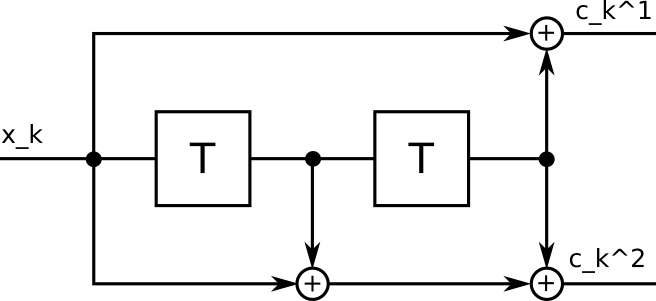
\includegraphics[scale=1.5]{images/convcodes_1_1.png}
\end{figure}


\subsection{Trellis Structure}

We can interpret the content of the $M$ shift registers as state (there are $2^M$ states) and the input values cause the values of the shift registers to change; i.e. state transitions. In addition, such a state transition produces an output (the $K$ values of $c_k^{(i)}$). The state transitions caused by inputs and the corresponding output can be visualized in a Trellis diagram. It shows the states (the content of the shift registers from left to right) before and after an input, with lines connecting the state transitions. A state transition is denoted by $b/c_1,\ldots c_k$.

The following Figure shows the Trellis diagram for the above code. For example, when in state $01$, an input $1$ causes a new state $10$ (the one from the input is shifted in from the left, causing the one on the right in the previous state to "falls out"), and an output of $00$.

\begin{figure}[h]
  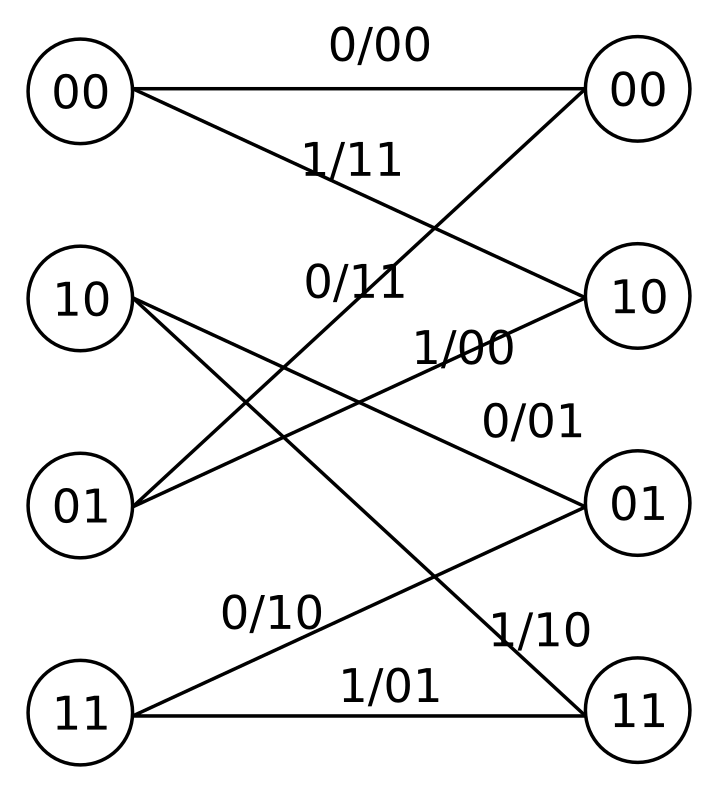
\includegraphics[scale=1.2]{images/convcodes_1_2.png}
\end{figure}



\subsection{Viterbi Decoding}

\subsubsection{Notation}

The information bit sequence $x_0, \ldots, x_{L-1}$ is denoted as vector $\xbf$. The vector of all $K$ code bits at time $k$ is denoted as $\cbf_k$ (the corresponding information bit is $x_k$); the sequence of all code bits is denoted as $\cbf$. For transmission, the code bits are mapped onto symbols $a$; for smplicity we assume a 1:1 mapping between code bits and symbols (e.g. BPSK). After the channel, the value $r$ is received. The received value corresponding to $\cbf_k$ is denoted as $\rbf_k$.

We consider two channel models, a BSC channel with 

\bee
r = a \oplus n, \quad n \sim \Bc(p)
\eee

where $\Bc$ is a Bernoulli random variable with crossover probability $p$ and $\oplus$ denotes addition modulo-$2$.

Second channel model is an AWGN with

\bee
r = a + n, \quad n \sim \Nc(0, \sigma_w^2)
\eee

with $n$ distributed normally with zero-mean and variance $\sigma_{w}^2$.

For both channels $n$ is assumed to iid; resulting in a memoryless channel. The sequence of transmitted symbols is denoted as $\abf$ and the received values is denoted as $\rbf$.

We denote the likelihood of the channels with $f(r|a)$, in case of a BSC we have

\bee
f(r|a) = \left( \frac{p_c}{1-p_c}\right)^{d_H(r,a)} (1-p_c)^n
\eee

where $d_H$ denotes the Hamming distance between two binary values. For the AWGN we have

\bee
f(r|a) = \frac{1}{(\sqrt{2\pi \sigma_w^2)^n}} \exp \left\{ - \frac{1}{2\sigma_w^2} (r - a)^2 \right\}
\eee

\subsubsection{Algorithm Description}

We want to find the maximum likelihood sequence; i.e. the sequence $\xbf$ which maximizes $f(\rbf|\xbf)$. Since there is a one-to-one correspondence between $\xbf$, $\cbf$, and $\abf$, $f(\rbf|\xbf) = f(\rbf|\cbf) = f(\rbf|\abf)$.

Maximizing the likelihood is equivalent to minimizing the metric; in case of the BSC the metric is $d_H(r,a)$; in case of the AWGN channel the metric is $(r-a)^2$.

The basic idea of the Viterbi algorithm is as follows. A sequence $\cbf$ (or, equivalently, $\abf$) corresponds to a path through the trellis. Due to channel noise, the received sequence may be different and the Viterbi decoder finds the sequence $\hat\cbf$ which is closest to the received $\rbf$ in terms of the metric (Hamming distance for the BSC, euclidean distance in case of the AWGN).

A naive approach would be to compute all paths through the trellis, calculate their metric (wrt to $\rbf$) and select the "closest" one. This is computationllay infeasible, as the number of paths grows exponentially with time.

The Viterbi algorithm is based on the observation that the path metric of a path can be expressed as sum of branch metrics and that all branch metrics are positive. This allows pruning of trellis paths and a big reduction in complexity.

We introduce the following notation: The sequence $\rbf_0,\ldots,\rbf_{L-1}$ is denoted as $\rbf_{0}^{L-1}$ and the sequence $x_0,\ldots,x_{L-1}$ is denoted as $\xbf_{0}^{L-1}$. The likelihood is

\bee
f(\rbf|\xbf) = f(\rbf_{0}^{L-1} | \rbf_{0}^{L-1}) = \prod_{i=0}^{L-1} f(\rbf_l|x_l)
\eee

which follows from the memoryless channel property. Considering log-likelihoods instead, we have

\bee
\log f(\rbf|\xbf) = \log f(\rbf_{0}^{L-1} | \rbf_{0}^{L-1}) = \sum_{i=0}^{L-1} \log f(\rbf_l|x_l)
\eee

Consider now a length-$N$ sequence $\xbf_{0}^{N-1}$ which leaves the trellis in state $\Psi_N = p$ at time $N$; the corresponding path through the trellis is denoted as $\Gamma_N = (\Psi_0,\ldots,\Psi_N)$. The negative log-likelihood of this sequence will be denoted as path metric $M_{N-1}(p)$ along the path $\Gamma_N$ and is given by

\bee
M_{N-1}(p) = - \log f(\rbf_{0}^{N-1} | \xbf_{0}^{N-1}) = - \sum_{i=0}^{N-1} \log f(r_i|x_i)
\eee

Now consider transmission of another information bit (in the next timeslot) and reception of a corresponding $\rbf_N$. We want to obtain the path metric along the path $\Gamma_N$ augmented by a new end state $q$; $\Gamma_{N+1} = (\Psi_0,\ldots,\Psi_N, q)$. The path metric for this longer path is then

\begin{align*}
M_N(q) & = - \sum_{i=0}^{N} \log f(\rbf_i|x_i) = - \sum_{i=0}^{N-1} \log f(\rbf_i|x_i) - f(\rbf_N|x_N) \\ &= M_{N-1}(p) - \log f(\rbf_N|x_N)
\end{align*}

This is the path metric of $\Gamma_N$ plus a path metric update caused by the state transition from $p$ to $q$.

The principle of the Viterbi algorithm is as follows: To obtain the shortest path through the trellis for the complete sequence $\xbf$, the path to every state in between must be the shortest. This is because the metric updates are strictly positive; i.e. a too large path metric cannot be reduced later on by a negative metric update.

This is relevant, when two paths merge into a state (see Figure below): Assume the two paths come from different states $p_1$ and $p_2$ and each has a different path metric $M_{N-1}(p_1)$ and $M_{N-1}(p_2)$, respectively. Observing the received value $\rbf_N$ allows calculating the path metric update as above (Note that the state transition from $p_1$ to $q$ and $p_2$ to $q$ is caused by a different $x_N$ and corresponidng $\cbf_N$). It is enough to retain only the path with the smaller metric, while the other path can be eliminated from futher consideration.


\begin{figure}[ht]
  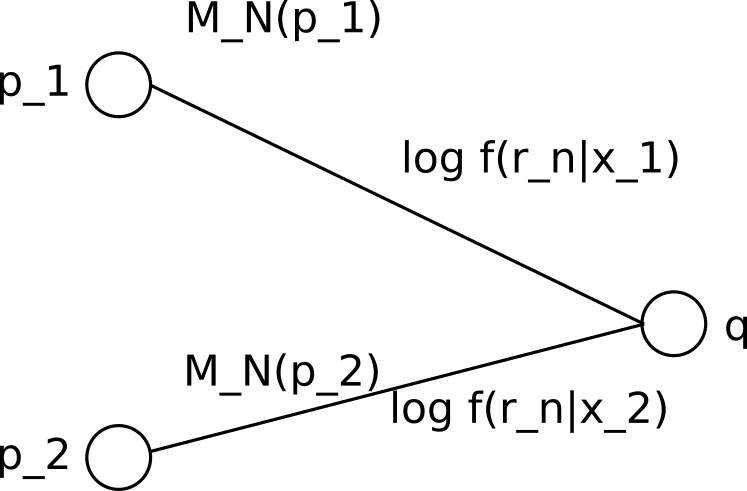
\includegraphics[scale=1.0]{images/convcodes_1_3.png}
\end{figure}

The Viterbi algorithm maintains the following data

\begin{itemize}

	\item A path metric to each state at time $t$.

	\item A path (list of states) to each state at time $t$.

\end{itemize}

The Viterbi algorithm therefore works as follows

\begin{enumerate}

\item Start with a list of empty paths to each state.

\item Start with an initial path metric $M(0) = 0$ and $M(p) = \infty, p \neq 0$. This ensures that the initial encoder state is $0$.

\item For each state $q$ at time $t$:

	\begin{enumerate}

		\item Find the path metric for each path to state $q$. According to the Figure above, there will be two candidate paths (with corresponding candidate path metrics).

		\item Choose the path the smaller metric.

		\item Extend the path by the chosen path.

		\item Update the path metric according to the chosen path.

	\end{enumerate}

\item Advance to the next time step

\item When done:

	\begin{itemize}

		\item When the encoder terminated in a known state (by zero-padding the information bit sequence), return the sequence of information bits along the path to that kown state.

		\item When the encoder terminated in any state known state, return the sequence of information bits along the path with the smallest metric.

	\end{itemize}

\end{enumerate}

%%% Local Variables:
%%% mode: latex
%%% TeX-master: "journal"
%%% End:
